\documentclass[a0paper,portrait]{article}
\usepackage{tikz}
\usepackage{geometry}
\geometry{margin=0cm} % Full page layout
\usetikzlibrary{calc}
\usepackage{lmodern} 


\begin{document}

\begin{tikzpicture}[remember picture, overlay]
    
    \newcommand{\marginwidth}{2cm}
    
    % Fill the entire page with navy blue
    \fill[blue!15!black] (current page.north west) rectangle (current page.south east);


     % Draw the inner white border (rectangle with no fill) symmetrically
     \draw[white, thick] 
        ([xshift=\marginwidth, yshift=-\marginwidth] current page.north west) 
        rectangle 
        ([xshift=-\marginwidth-0.5cm, yshift=\marginwidth] current page.south east);

    
   % define location of title
       \coordinate (Titleloc) at ([xshift=\marginwidth, yshift=-1cm] current page.north west);
       
    %define location of logo
    \coordinate (logoloc) at ([xshift=12cm, yshift=-8cm] current page.north west);

    % Draw a white background box for the logo (if the logo has non-transparent background)
    \node[anchor=east, fill=white, minimum width=9.5cm, minimum height=11cm] at (logoloc) {};
    
    
    % Add a logo to the left side of the title
    \node[anchor=east] at (logoloc) 
        {
\includegraphics[width=9cm]{logo.png}}; % Adjust logo size as needed

    %Title
    \node[cyan!70!white, font=\fontsize{74}{70}\bfseries, align=center] 
        at (Titleloc) [xshift=+44.5cm,yshift=-5cm] 
        {A Deep Learning Pipeline for Genome-Wide Imaging \\ Screen Uncovering 
        Cell Death Regulators};

    %Define name location    
 \coordinate (nameloc) at ([xshift=12cm, yshift=-16cm] current page.north west);

 %define names
 \node[white, font=\fontsize{54}{30}\bfseries, align=center] 
        at (nameloc) [xshift=+34cm,yshift=4cm] 
        {Salma Kazemi Rashed, Klara Esbo, Mariam Miari, Malou Arvidsson, \\ Liu J, Cowley K, Simpson K, Johnstone R, Sonja Aits
};

\node[white!80!cyan, font=\fontsize{44}{30}\bfseries, align=center] 
        at (nameloc) [xshift=+34cm,yshift=0cm] 
        {Cell Death, Lysosomes and AI group, Lund University, Email: $Salma.kazemi\_rashed@med.lu.se$
};



% Calculate the coordinates of the big white circle
    \coordinate (center) at ([xshift=-52cm, yshift=-63cm]current page.center);
    
    % Draw a filled white half circle (right half) inside the inner rectangle
    \fill[white!90!black] 
        (center) arc[start angle=270, end angle=450, radius=55cm];

    % Introduction
    \node[orange, font=\fontsize{54}{30}\bfseries, align=center] at (center) [xshift=18cm,yshift=102cm]  {Introduction};
    %orange hline 
    \draw[orange,line width=3mm] 
        ([xshift=2cm, yshift=-22cm] current page.north west) 
        -- ([xshift=18cm, yshift=-22cm] current page.north west);
    

    % Line at -45 degrees angle with color orange
    \draw[orange, line width=3mm] 
        ([xshift=18cm, yshift=-22cm] current page.north west) 
        -- ++(-45:12cm); % 45 degrees and 5cm length

    %Introduction text
     \node[blue!20!black,font=\fontsize{31}{30}\bfseries, text width=16cm, align=justify] at (center) [xshift=20cm,yshift=91cm] {Cell death is a crucial biological process that creates space for new cells and prevents the spread of harmful mutated cells. It is highly regulated, but mutations in regulatory genes can lead to excessive or insufficient cell death, contributing to various diseases. There are different types of cell death, including a regulated process where the cell fragments and an uncontrolled one triggered by trauma, causing the cell to swell and burst.};

       \node[blue!20!black,font=\fontsize{31}{30}\bfseries, text width=24cm, align=justify] at (center) [xshift=24cm,yshift=79cm] { Cell death process can alter the nucleus, cell body, and organelles like lysosomes, which contain harmful enzymes. Lysosomal membrane permeabilization (LMP) can trigger cell death and affect other organelles like mitochondria (MMP).};


 \node[orange,font=\fontsize{38}{30}\bfseries,align=justify] at (center) [xshift=17cm,yshift=74.5cm] { Nuclei };

\node[blue!20!black,font=\fontsize{38}{30}\bfseries,align=justify] at (center) [xshift=17cm,yshift=57cm] { Swollen };


  \node[orange,font=\fontsize{38}{30}\bfseries,align=justify] at (center) [xshift=27.5cm,yshift=74.5cm] { Lysosome};

\node[blue!20!black,font=\fontsize{38}{30}\bfseries,align=justify] at (center) [xshift=28cm,yshift=57cm] { LMP };

   \node[orange,font=\fontsize{38}{30}\bfseries,align=justify] at (center) [xshift=39cm,yshift=74.5cm] { Mitochondria };

   \node[blue!20!black,font=\fontsize{38}{30}\bfseries,align=justify] at (center) [xshift=39cm,yshift=57cm] { MMP };
     %define location of cell death
    \coordinate (cellloc) at ([xshift=12cm, yshift=-52cm] current page.north west);


     \node[anchor=east] at (cellloc)  [xshift=0cm, yshift=-2cm]
        {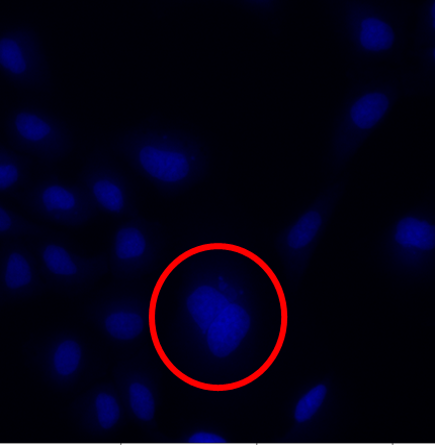
\includegraphics[ width=10cm]{nuclei.png}};
     \node[anchor=east] at (cellloc) [xshift=11cm, yshift=-2cm]
        {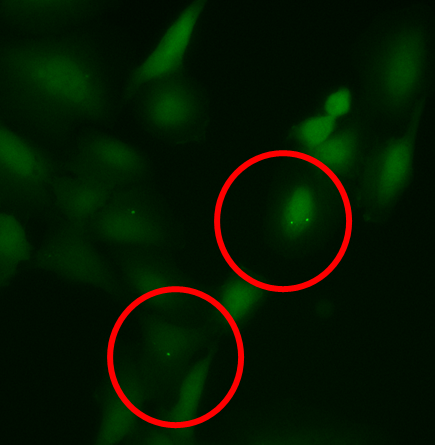
\includegraphics[ width=10cm]{cytosol.png}};

     \node[anchor=east] at (cellloc) [xshift=22cm, yshift=-2cm]
        {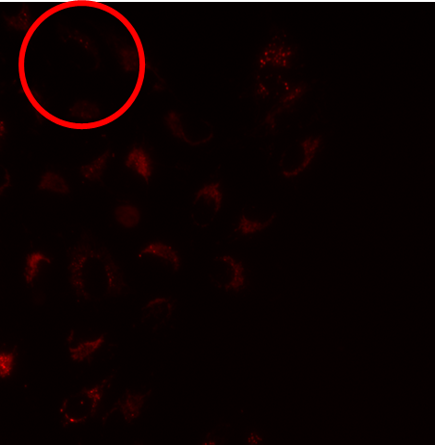
\includegraphics[ width=10cm]{mitho.png}};
    


    %cartoons
    \node[anchor=east] at (cellloc)  [xshift=-2.5cm, yshift=-10cm]
        {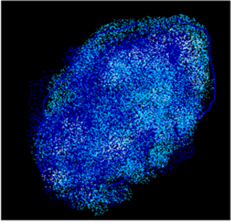
\includegraphics[ width=5cm]{swell_nuclei.png}};

     \node[anchor=east] at (cellloc)  [xshift=8.5cm, yshift=-10cm]
        {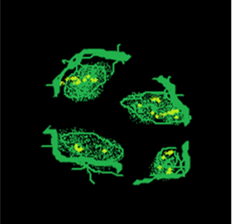
\includegraphics[ width=5cm]{LMP.png}};
 

     \node[anchor=east] at (cellloc)  [xshift=19.5cm, yshift=-10cm]
        {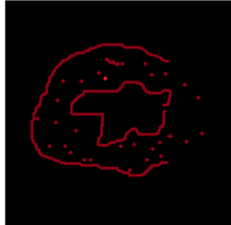
\includegraphics[ width=5cm]{mitho_cartoon.png}};
    % Add a nuclei to here
 
%Text for cell death  
\node[blue!20!black,font=\fontsize{38}{30}\bfseries,align=justify] at (center) [xshift=28cm,yshift=55cm] { Cell death};





% Calculate the coordinates of the big white circle
    \coordinate (center) at ([xshift=0cm, yshift=30cm]current page.center);
    
    % Draw a filled white half circle (right half) inside the inner rectangle
    \fill[orange] 
        (center) arc[start angle=0, end angle=360, radius=11cm];
        
   \coordinate (whitecenter) at ([xshift=-2cm, yshift=30cm]current page.center);
    
    % Draw a filled white half circle (right half) inside the inner rectangle
    \fill[white] 
        (whitecenter) arc[start angle=0, end angle=360, radius=9cm];

   
    
    % Draw a filled white half circle (right half) inside the inner rectangle
   

 \begin{scope}
        \clip (30.5,-29) circle(9cm);
        \node at (30.5,-29) {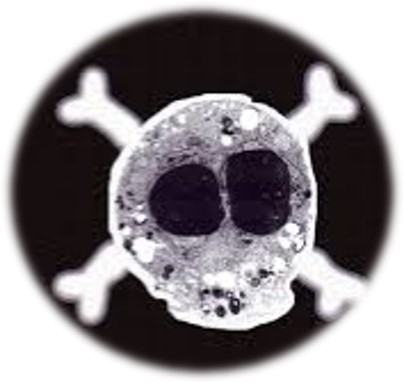
\includegraphics[width=16cm]{cell_death.png}};
    \end{scope}

%second circle

% Calculate the coordinates of the big white circle
    \coordinate (pinkcenter) at ([xshift=12cm, yshift=22cm]current page.center);
    
    % Draw a filled white half circle (right half) inside the inner rectangle
    \fill[pink] 
        (pinkcenter) arc[start angle=0, end angle=360, radius=10cm];
        
   \coordinate (whitepinkcenter) at ([xshift=10cm, yshift=22cm]current page.center);
    
    % Draw a filled white half circle (right half) inside the inner rectangle
    \fill[white] 
        (whitepinkcenter) arc[start angle=0, end angle=360, radius=8cm];

   
    
    % Draw a filled white half circle (right half) inside the inner rectangle
  
\begin{scope}
        \clip (43.5,-37) circle(7cm);
        \node at (43.5,-37) {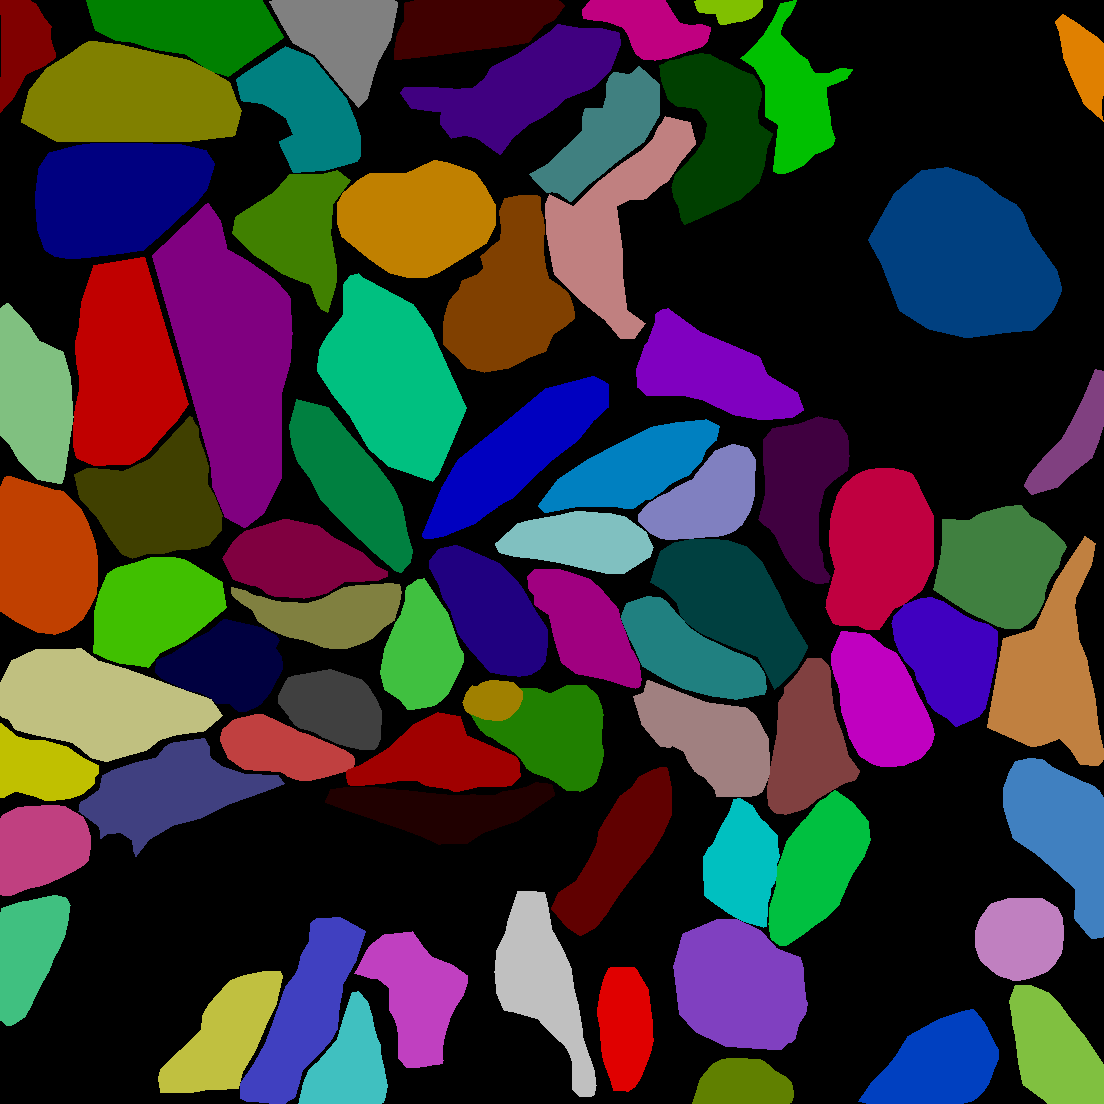
\includegraphics[width=16cm]{Annotation.png}};
    \end{scope}





%third circle
    \coordinate (cyancenter) at ([xshift=11cm, yshift=9cm]current page.center);
    \fill[cyan!40!white] 
        (cyancenter) arc[start angle=0, end angle=360, radius=8cm];
        
   \coordinate (whitecyancenter) at ([xshift=10cm, yshift=9cm]current page.center);
    
    % Draw a filled white half circle (right half) inside the inner rectangle
    \fill[white] 
        (whitecyancenter) arc[start angle=0, end angle=360, radius=7cm];

    
    % Draw a filled white half circle (right half) inside the inner rectangle
  
\begin{scope}
        \clip (44.5,-50) circle(6cm);
        \node at (44.5,-50) {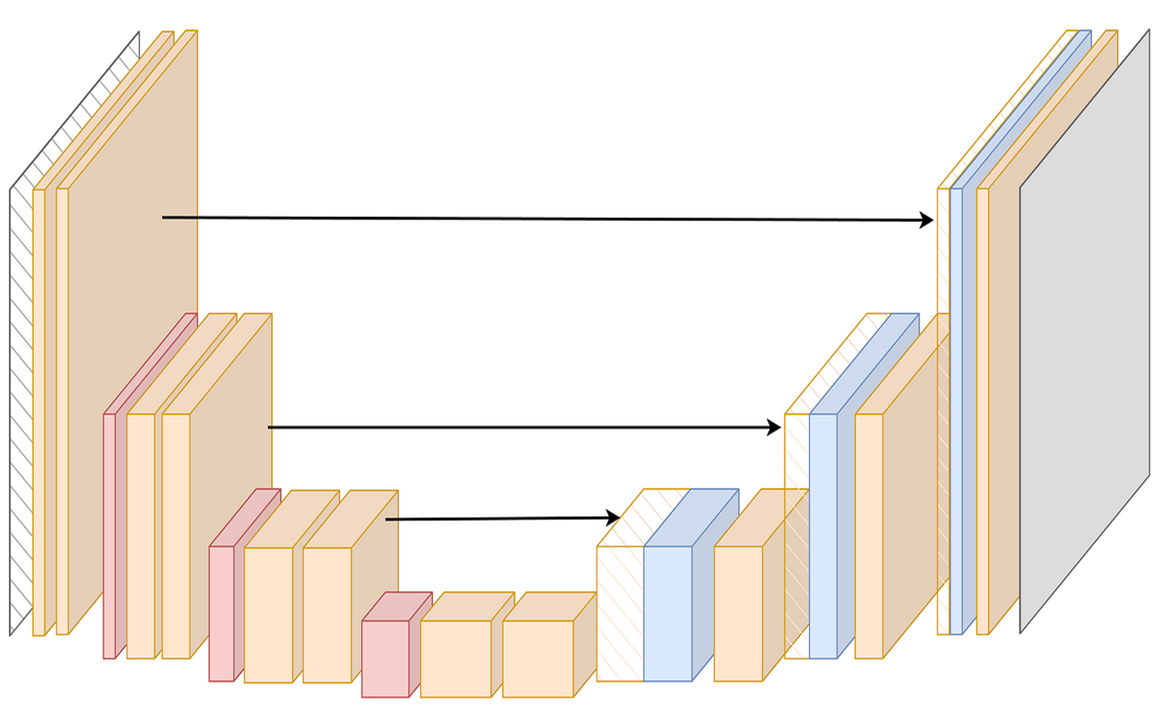
\includegraphics[clip,trim=0cm 0cm 0cm 0cm,width=12cm]{UNet.png}};
    \end{scope}




%fourth circle
    \coordinate (torqcenter) at ([xshift=12cm, yshift=-6cm]current page.center);
    \fill[green!40!blue] 
        (torqcenter) arc[start angle=0, end angle=360, radius=9cm];
        
   \coordinate (whitetorqcenter) at ([xshift=11cm, yshift=-6cm]current page.center);
    
    % Draw a filled white half circle (right half) inside the inner rectangle
    \fill[white] 
        (whitetorqcenter) arc[start angle=0, end angle=360, radius=8cm];

    
    % Draw a filled white half circle (right half) inside the inner rectangle
  
\begin{scope}
        \clip (44.5,-65) circle(7cm);
        \node at (44.5,-65) {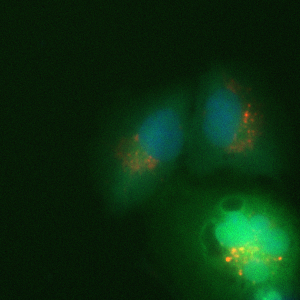
\includegraphics[clip,trim=2cm 0cm 0cm 0cm,width=16cm]{healthy.png}};
    \end{scope}



%fifth circle
    \coordinate (browncenter) at ([xshift=12cm, yshift=-25cm]current page.center);
    \fill[brown!60!white] 
        (browncenter) arc[start angle=0, end angle=360, radius=9cm];
        
   \coordinate (whitebrowncenter) at ([xshift=11cm, yshift=-25cm]current page.center);
    
    % Draw a filled white half circle (right half) inside the inner rectangle
    \fill[white] 
        (whitebrowncenter) arc[start angle=0, end angle=360, radius=8cm];

    
    % Draw a filled white half circle (right half) inside the inner rectangle
  
\begin{scope}
        \clip (44.5,-84) circle(7cm);
        \node at (44.5,-84) {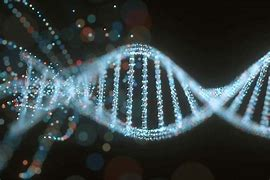
\includegraphics[clip,trim=2cm 0cm 0cm 0cm,width=18cm]{genome.png}};
    \end{scope}

%6th circle
    \coordinate (greencenter) at ([xshift=-6cm, yshift=-43cm]current page.center);
    \fill[cyan!40!green] 
        (greencenter) arc[start angle=0, end angle=360, radius=8cm];
        
   \coordinate (whitegreencenter) at ([xshift=-7cm, yshift=-43cm]current page.center);
    
    % Draw a filled white half circle (right half) inside the inner rectangle
    \fill[white] 
        (whitegreencenter) arc[start angle=0, end angle=360, radius=7cm];

    
    % Draw a filled white half circle (right half) inside the inner rectangle
  
\begin{scope}
        \clip (27.5,-102) circle(6cm);
        \node at (27.5,-102) {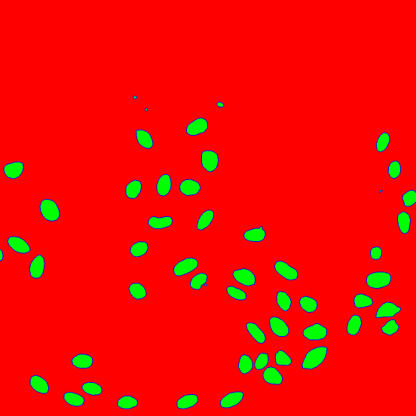
\includegraphics[clip,trim=0cm 0cm 0cm 0cm,width=18cm]{annot.png}};
    \end{scope}






% Dataset
    \node[green!40!blue, font=\fontsize{54}{30}\bfseries, align=center] at (center) [xshift=-36cm,yshift=-40cm]  {Dataset};
    %orange hline 
    \draw[green!40!blue,line width=3mm] 
        ([xshift=2cm, yshift=-71cm] current page.north west) 
        -- ([xshift=30cm, yshift=-71cm] current page.north west);
    

    % Line at -45 degrees angle with color orange
    \draw[green!40!blue, line width=3mm] 
        ([xshift=30cm, yshift=-71cm] current page.north west) 
        -- ++(45:10cm); % 45 degrees and 5cm length

    %Introduction text
     \node[blue!20!black,font=\fontsize{31}{30}\bfseries, text width=35cm, align=justify] at (center) [xshift=-22.5cm,yshift=-46.5cm] {The dataset comprises 4,276,224 image frames (1104x1104x3), collected from a gene knockdown study on U2OS osteosarcoma cells, conducted by Dr. Sonja Aits. Cells were transfected with an siRNA library targeting 18,170 protein-coding genes, and phenotypic changes were visualized across 213 plates using three fluorescent channels to label key cell components. The nucleus was labelled by Hoechst 33342, cells by EGFP-LGALS3, and mitochondria channel by Omi-mcherry staining.
};



     \node[anchor=east] at (cellloc)  [xshift=23cm, yshift=-35cm]
        {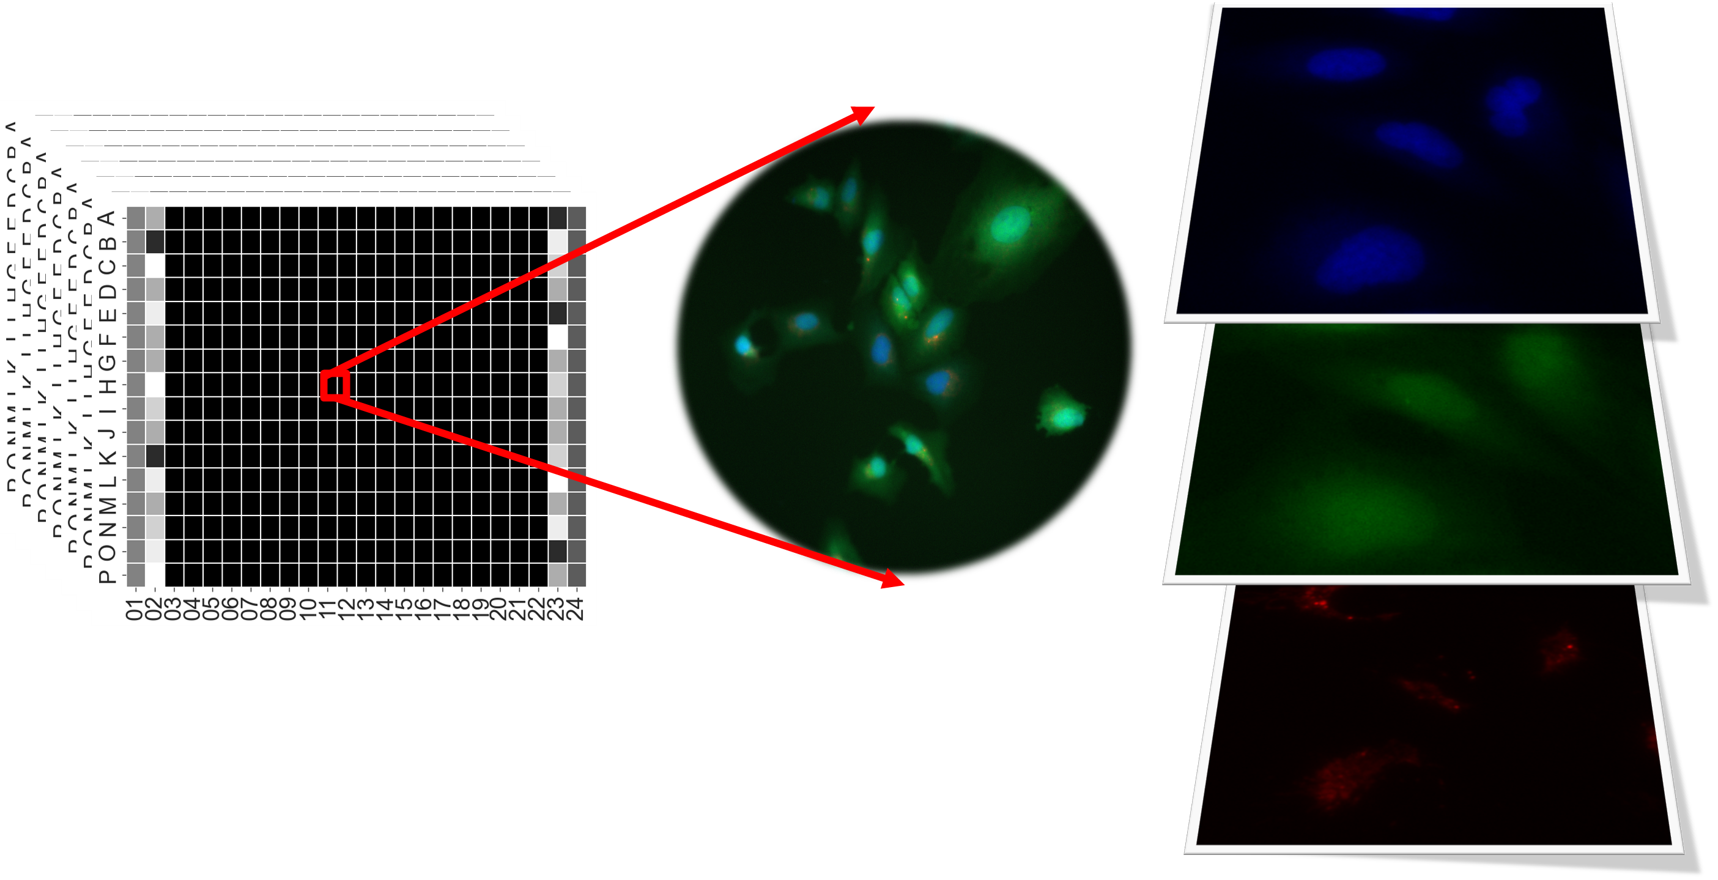
\includegraphics[ width=30cm]{dataset_new.png}};


\node[blue
,font=\fontsize{31}{30}\bfseries,align=justify] at (center) [xshift=-13cm,yshift=-52cm] {Hoechst 33342};

\node[green!70!blue,font=\fontsize{31}{30}\bfseries,align=justify] at (center) [xshift=-12cm,yshift=-58cm] {EGFP-LGALS3
};

\node[red!70!black,font=\fontsize{31}{30}\bfseries,align=justify] at (center) [xshift=-12cm,yshift=-62cm] {Omi-mcherry
};


\node[blue!20!black,font=\fontsize{36}{30}\bfseries,align=justify] at (center) [xshift=-24cm,yshift=-62cm] {Osteosarcoma Cells

};

 \node[cyan!40!green, font=\fontsize{54}{30}\bfseries, align=center] at (current page.north west) [xshift=7.5cm,yshift=-96cm]  {Annotation};
    %orange hline 
    \draw[cyan!40!green,line width=3mm] 
        ([xshift=2cm, yshift=-98cm] current page.north west) 
        -- ([xshift=22cm, yshift=-98cm] current page.north west);
        
     \node[blue!20!black,font=\fontsize{31}{30}\bfseries, text width=15 cm, align=justify] at (center) [xshift=-32.5cm,yshift=-73cm] {We manually annotated a small subset of our dataset, consisting of 50 images: 30 for training, 10 for validation, and 10 for testing the model before applying it to the full dataset [1][2].
};

% Objective
    \node[pink, font=\fontsize{54}{30}\bfseries, align=center] at (center) [xshift=34cm,yshift=9cm]  {Objective};
    %orange hline 
    \draw[pink,line width=3mm] 
        ([xshift=39cm, yshift=8cm] center) 
        -- ([xshift=9cm, yshift=8cm] center);
    

    % Line at -45 degrees angle with color orange
    \draw[pink, line width=3mm] 
        ([xshift=9cm, yshift=8cm] center) 
        -- ++(-135:11cm); % 45 degrees and 5cm length

    %Introduction text
     \node[pink!20!white,font=\fontsize{31}{30}\bfseries, text width=30cm, align=justify] at (center) [xshift=24cm,yshift=3cm] {This study focuses on cell nuclei, extracting morphological features of all nuclear objects in order to find dying or dead cells, such as shape, area, and count. Using a genome-wide knockdown experiment, where each human gene was silenced and corresponding cell images were captured, these features are linked to the genome to identify cell death pathways.
};


%Methodolgy
   \node[cyan!40!white, font=\fontsize{54}{30}\bfseries, align=center] at (center) [xshift=33cm,yshift=-5cm]  {Methodology};
    %orange hline 
    \draw[cyan!40!white,line width=3mm] 
        ([xshift=39cm, yshift=-6cm] center) 
        -- ([xshift=12cm, yshift=-6cm] center);
    

    % Line at -45 degrees angle with color orange
    \draw[cyan!40!white, line width=3mm] 
        ([xshift=12cm, yshift=-6cm] center) 
        -- ++(-135:11cm); % 45 degrees and 5cm length

    %Introduction text
     \node[cyan!10!white,font=\fontsize{31}{30}\bfseries, text width=26cm, align=justify] at (center) [xshift=26cm,yshift=-13cm] {The nearly 9 TB dataset of over 213 plates lacked annotations, prompting a stepwise solution. We manually annotated 50 images from nuclei[1], and cell[2] channels and utilized public datasets, such as the Broad Bioimage Benchmark Collection (BBBC), to train U-Net models from scratch, and experimented with advanced models like Hover-Net leveraging transfer learning. The best model achieved 89\% F1-score and was applied to the entire dataset to segment nuclei and extract size and count features.
};


%Results
   \node[cyan!40!green, font=\fontsize{54}{30}\bfseries, align=center] at (center) [xshift=35cm,yshift=-22cm]  {Results};
    %orange hline 
    \draw[cyan!40!green,line width=3mm] 
        ([xshift=39cm, yshift=-23cm] center) 
        -- ([xshift=13cm, yshift=-23cm] center);
    

   
    %Introduction text
     \node[green!10!white,font=\fontsize{31}{30}\bfseries, text width=26cm, align=justify] at (center) [xshift=26cm,yshift=-28cm] {We evaluated using F1-score and Jaccard Index, with IoU (
$IOU(A,B) = \dfrac {A \cap B }{A\cup B}$
 ) measuring overlap between predictions and annotations. F1-score, an object-based metric calculated as the geometric mean of recall and precision, was assessed at IoU thresholds ranging from 50\% to 90\%, with the final evaluation at 90\%.
};


     \node[anchor=east] at (cellloc)  [xshift=68cm, yshift=-18cm]
        {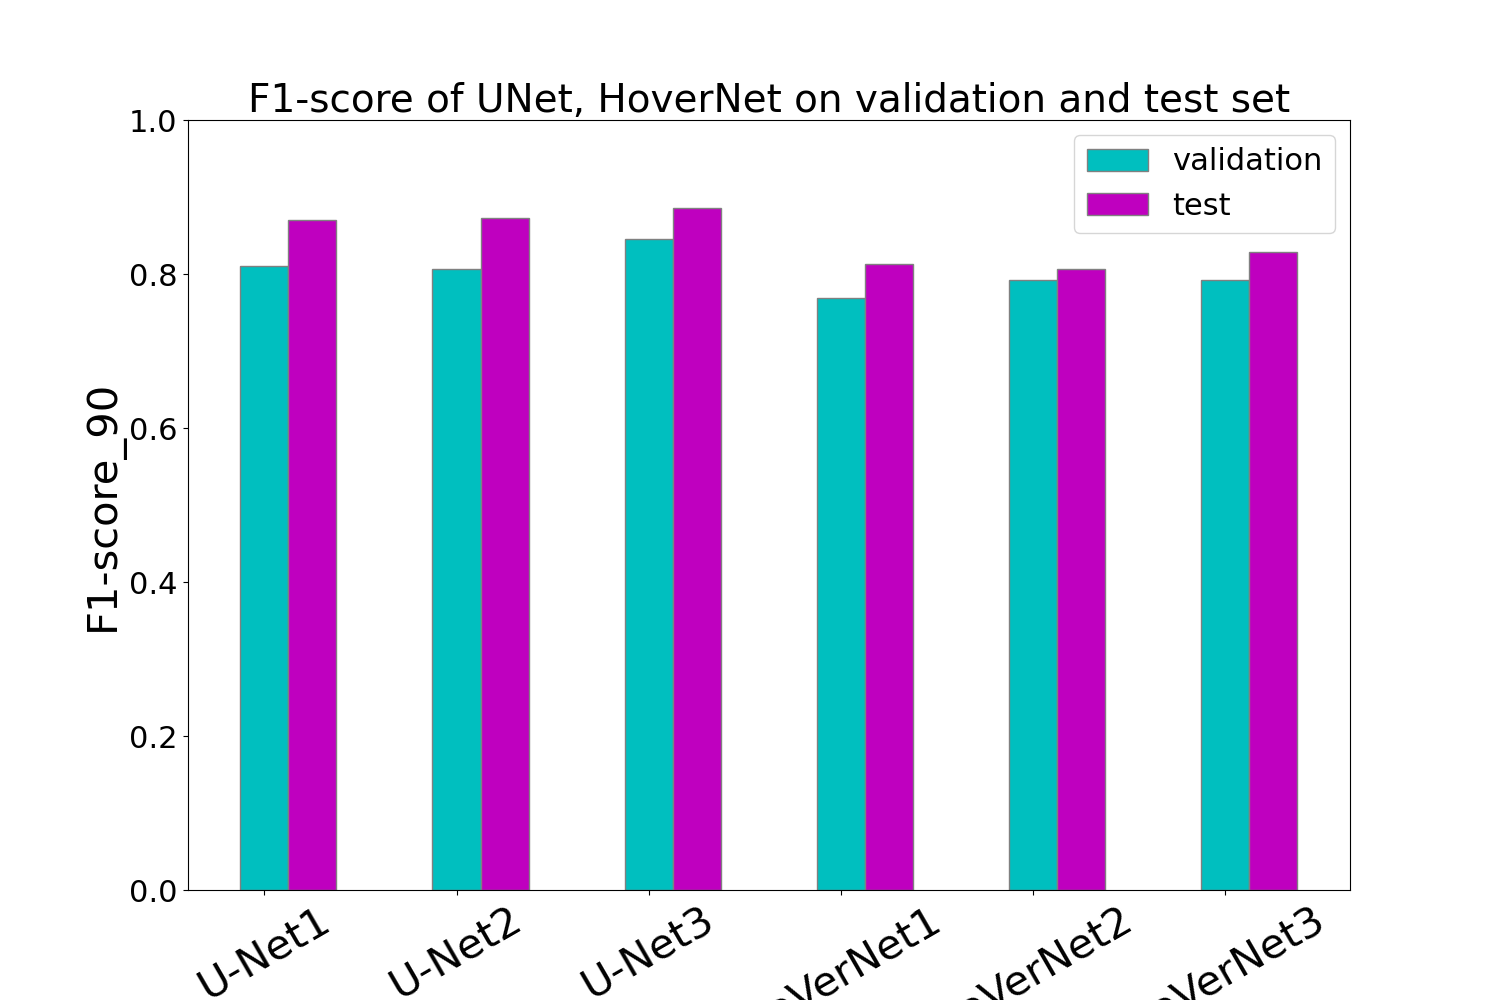
\includegraphics[ clip,trim=1cm 0cm 3cm 0cm,width=21cm]{F1_score_val_test.png}};

    %Results
   \node[brown!60!white, font=\fontsize{54}{30}\bfseries, align=center] at (center) [xshift=29cm,yshift=-50cm]  {Genome-wide screen};
    %orange hline 
    \draw[brown!60!white,line width=3mm] 
        ([xshift=39cm, yshift=-51cm] center) 
        -- ([xshift=11cm, yshift=-51cm] center);

      \node[brown!20!white,font=\fontsize{31}{30}\bfseries, text width=26cm, align=justify] at (center) [xshift=26cm,yshift=-53.5cm] { 
The best model was applied to the full dataset, and the nuclei count and area for each well were plotted.
};
    
     \node[anchor=east] at (cellloc)  [xshift=68cm, yshift=-39cm]
        {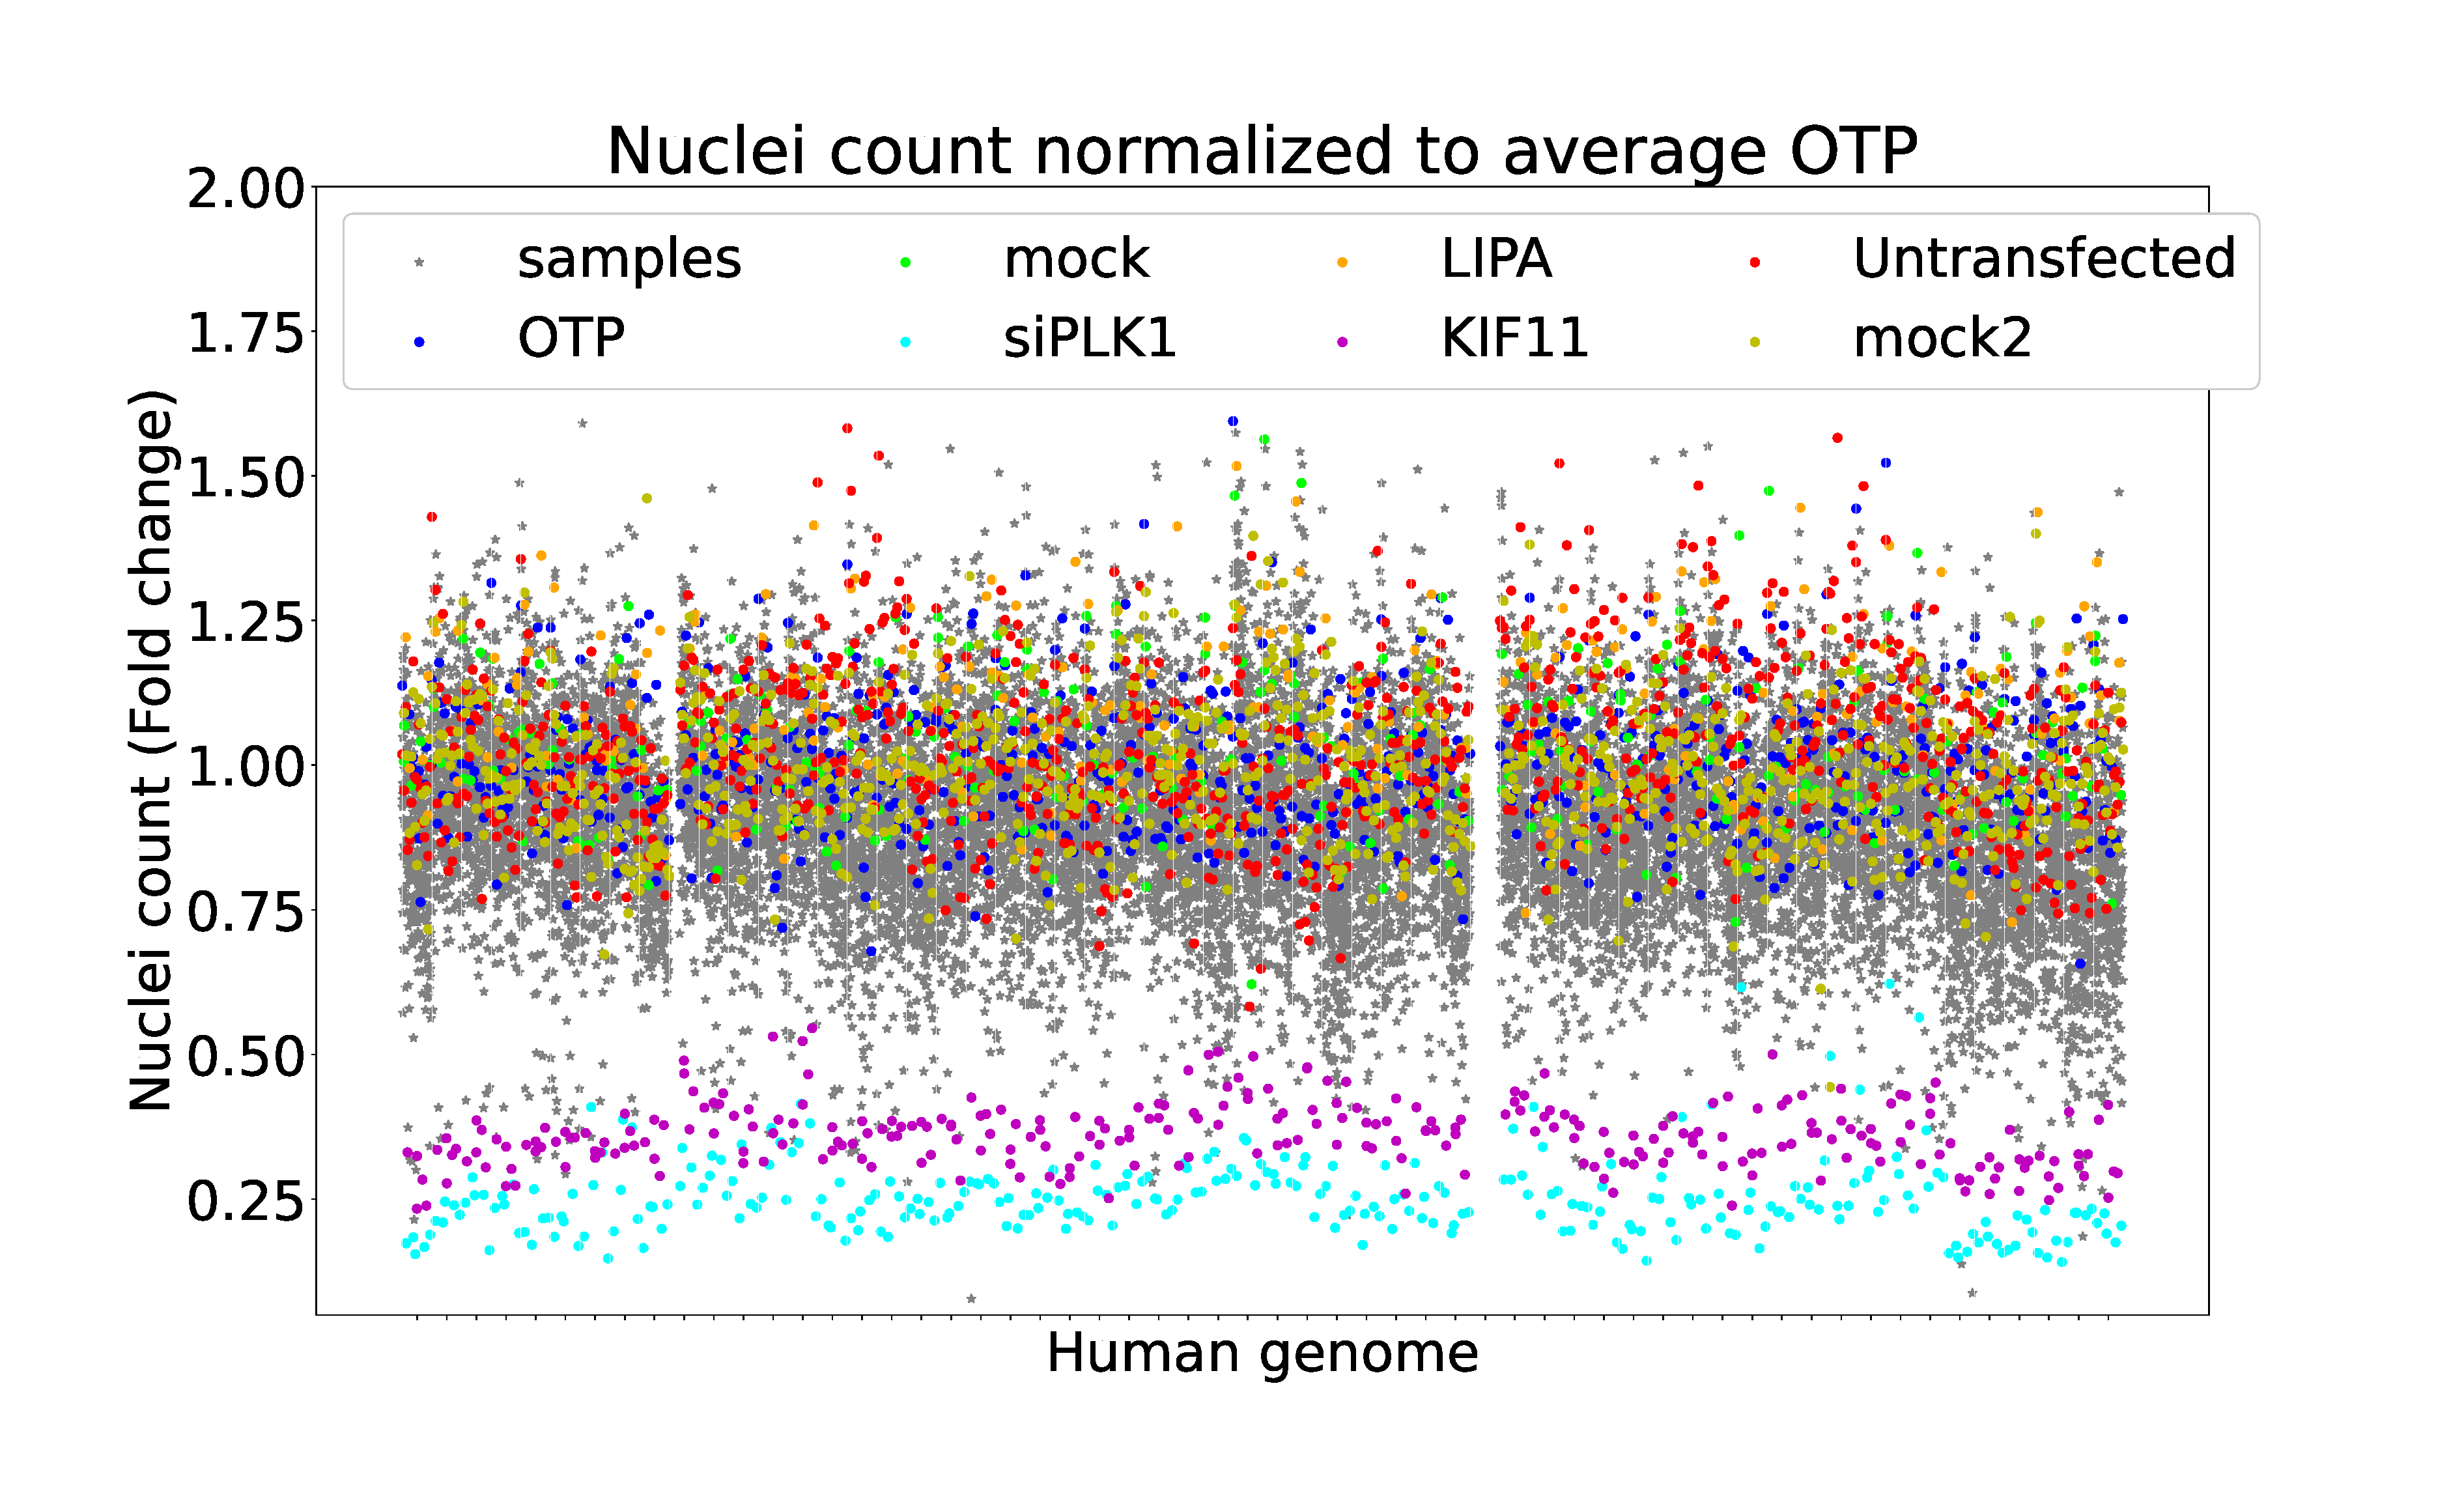
\includegraphics[ clip,trim=1cm 0cm 3cm 0cm,width=21cm]{Nuclei_count.eps}};

        
     \node[anchor=east] at (cellloc)  [xshift=68cm, yshift=-52cm]
        {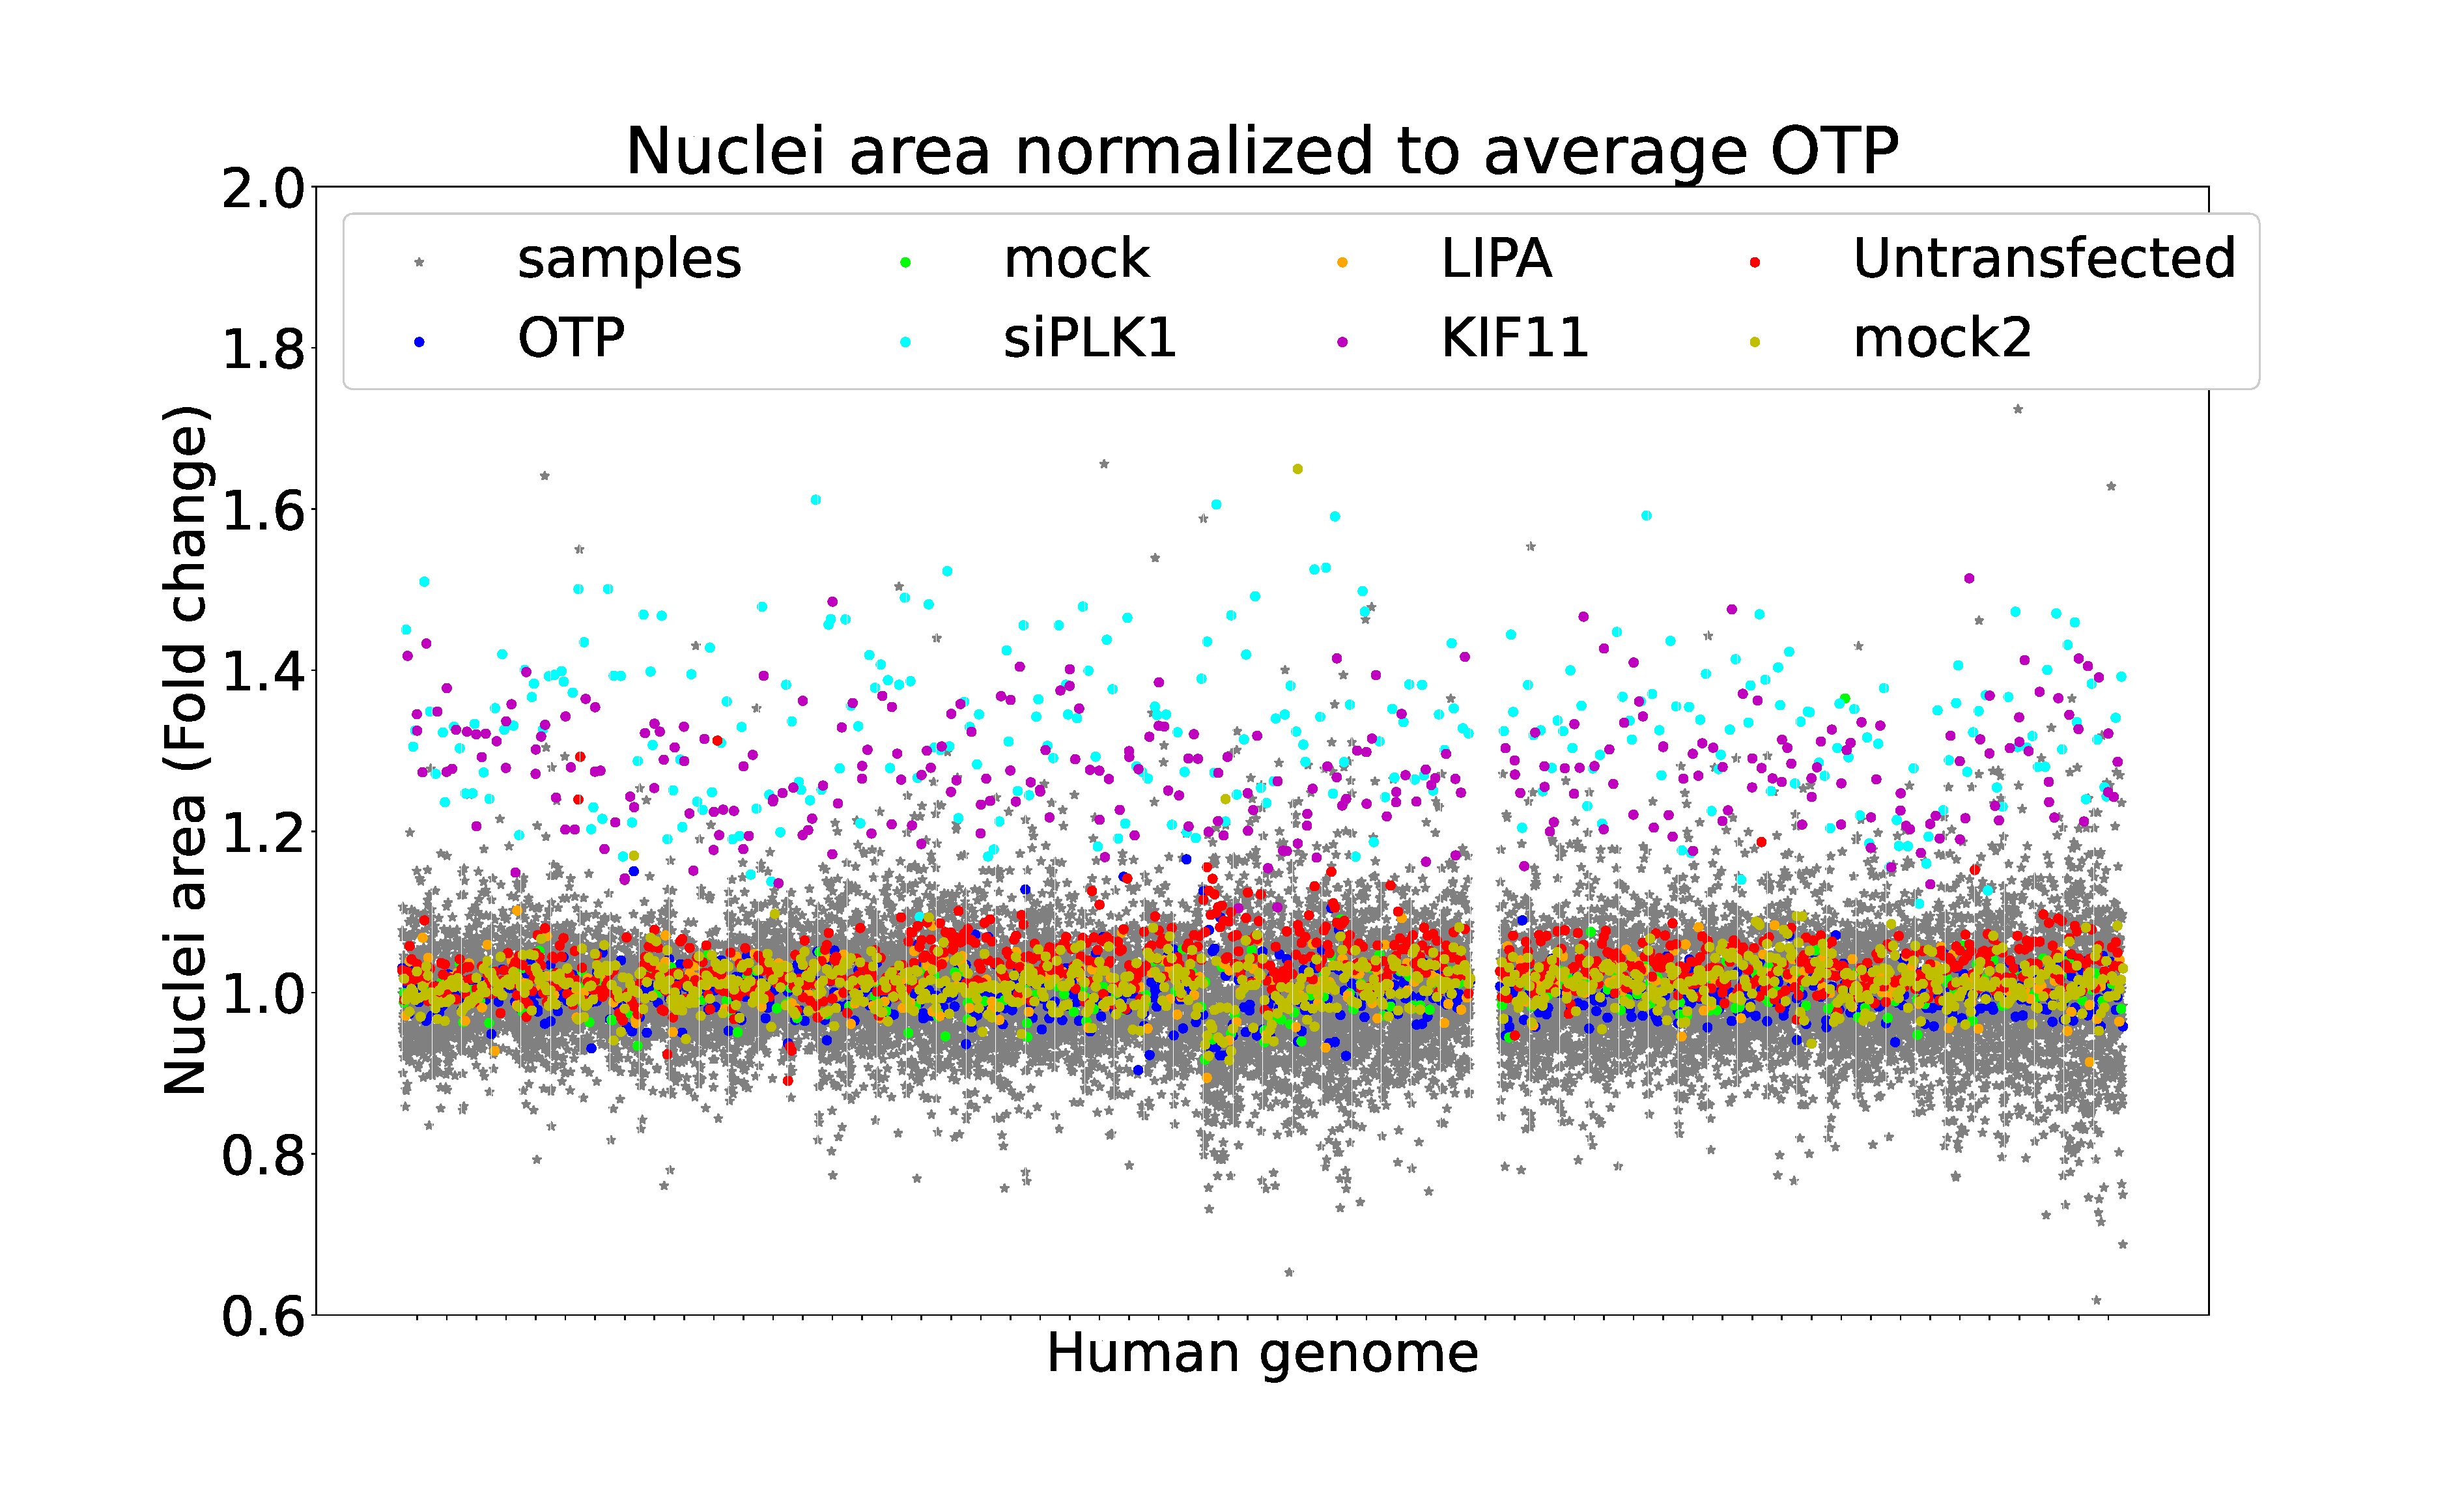
\includegraphics[ clip,trim=1cm 0cm 3cm 0cm,width=21cm]{Nuclei_area.eps}};


  %Results
   \node[brown!70!black, font=\fontsize{54}{30}\bfseries, align=center] at (center) [xshift=9cm,yshift=-66cm]  {Conclusion};
    %orange hline 
    \draw[brown!70!black,line width=3mm] 
        ([xshift=15cm, yshift=-67cm] center) 
        -- ([xshift=-4cm, yshift=-67cm] center);

     \node[brown!20!white,font=\fontsize{31}{30}\bfseries, text width=20cm, align=justify] at (center) [xshift=5cm,yshift=-70cm] {
Identifying wells with significant nuclei changes allowed us to link them to genes, resulting in a list of candidates for further study in novel cell death pathways.}



\node[brown!40!white,anchor=south east] at (current page.south east) [xshift=-27cm, yshift=8cm] {
\resizebox{20cm}{!}{
\begin{tabular}{|c|c|c|}
\hline
\textbf{Gene}&{\textbf{Count}} &{\textbf{Area}} \\  
\hline

FBXO5 &   $< 0.5 \quad$  &   $ \quad > 1.7$  \\
\hline
CCNA2 & $< 0.5 \quad$  &   $ \quad > 1.7$  \\
\hline
UBB  & $< 0.1 \quad$  &     \\
\hline
POLR2A &$< 0.1 \quad$  &   \\
\hline

\end{tabular}
}
};

     \node[brown!50!white,font=\fontsize{20}{30}\bfseries, text width=76cm, align=justify] at (current page.south) [xshift=-2cm,yshift=6cm] {[1] Malou Arvidsson, Salma Kazemi Rashed, Sonja Aits, An annotated high-content fluorescence microscopy dataset with Hoechst 33342-stained nuclei and manually labelled outlines, Data in Brief,  Volume 46,  2023, 108769, ISSN 2352-3409, https://doi.org/10.1016/j.dib.2022.108769.

};


     \node[brown!50!white,font=\fontsize{20}{30}\bfseries, text width=76cm, align=justify] at (current page.south) [xshift=-2cm,yshift=3.5cm] {[2] Salma Kazemi Rashed, Malou Arvidsson, Rafsan Ahmed, Sonja Aits,
An annotated high-content fluorescence microscopy dataset with EGFP-Galectin-3-stained cells and manually labelled outlines,
Data in Brief,
2024,
111148,
ISSN 2352-3409,
https://doi.org/10.1016/j.dib.2024.111148.

};



    \end{tikzpicture}





\end{document}


\end{document}
